%%%%%%%%%%%%%%%%%%%%%%%%%%%%%%%%%%%%%%%%%
% University Assignment Title Page 
% LaTeX Template
% Version 1.0 (27/12/12)
%
% This template has been downloaded from:
% http://www.LaTeXTemplates.com
%
% Original author:
% WikiBooks (http://en.wikibooks.org/wiki/LaTeX/Title_Creation)
%
% License:
% CC BY-NC-SA 3.0 (http://creativecommons.org/licenses/by-nc-sa/3.0/)
% 
% Instructions for using this template:
% This title page is capable of being compiled as is. This is not useful for 
% including it in another document. To do this, you have two options: 
%
% 1) Copy/paste everything between \begin{document} and \end{document} 
% starting at \begin{titlepage} and paste this into another LaTeX file where you 
% want your title page.
% OR
% 2) Remove everything outside the \begin{titlepage} and \end{titlepage} and 
% move this file to the same directory as the LaTeX file you wish to add it to. 
% Then add \input{./title_page_1.tex} to your LaTeX file where you want your
% title page.
%
%%%%%%%%%%%%%%%%%%%%%%%%%%%%%%%%%%%%%%%%%

%----------------------------------------------------------------------------------------
%	PACKAGES AND OTHER DOCUMENT CONFIGURATIONS
%----------------------------------------------------------------------------------------

\documentclass[12pt]{article}

\usepackage[utf8]{inputenc}
\usepackage[T1]{fontenc}
\usepackage{lmodern}
\usepackage{parselines}
\usepackage[portuguese]{babel}
\usepackage{graphicx}
\usepackage[document]{ragged2e}
\usepackage{listings}
\usepackage{xcolor}
\usepackage[margin=0.8in]{geometry}		
\usepackage{amsmath}
\usepackage{hyperref}
\usepackage{url}
\usepackage{float}
\usepackage{tabularx}
\usepackage{booktabs}

\graphicspath{ {images/} }

\colorlet{punct}{red!60!black}
\definecolor{background}{HTML}{EEEEEE}
\definecolor{delim}{RGB}{20,105,176}
\colorlet{numb}{magenta!60!black}


\lstdefinelanguage{json}{
    basicstyle=\normalfont\ttfamily,
    numbers=left,
    numberstyle=\scriptsize,
    stepnumber=1,
    numbersep=8pt,
    showstringspaces=false,
    breaklines=true,
    frame=lines,
    backgroundcolor=\color{background},
    literate=
     *{0}{{{\color{numb}0}}}{1}
      {1}{{{\color{numb}1}}}{1}
      {2}{{{\color{numb}2}}}{1}
      {3}{{{\color{numb}3}}}{1}
      {4}{{{\color{numb}4}}}{1}
      {5}{{{\color{numb}5}}}{1}
      {6}{{{\color{numb}6}}}{1}
      {7}{{{\color{numb}7}}}{1}
      {8}{{{\color{numb}8}}}{1}
      {9}{{{\color{numb}9}}}{1}
      {:}{{{\color{punct}{:}}}}{1}
      {,}{{{\color{punct}{,}}}}{1}
      {\{}{{{\color{delim}{\{}}}}{1}
      {\}}{{{\color{delim}{\}}}}}{1}
      {[}{{{\color{delim}{[}}}}{1}
      {]}{{{\color{delim}{]}}}}{1},
}

\definecolor{dkgreen}{rgb}{0,0.6,0}
\definecolor{gray}{rgb}{0.5,0.5,0.5}
\definecolor{mauve}{rgb}{0.58,0,0.82}

\lstset{frame=tb,
  language=Java,
  aboveskip=3mm,
  belowskip=3mm,
  showstringspaces=false,
  columns=flexible,
  basicstyle={\small\ttfamily},
  numbers=none,
  numberstyle=\tiny\color{gray},
  keywordstyle=\color{blue},
  commentstyle=\color{dkgreen},
  stringstyle=\color{mauve},
  breaklines=true,
  breakatwhitespace=true,
  tabsize=3
}

\hypersetup{
  colorlinks, linkcolor=black
}

\begin{document}

\begin{titlepage}

\newcommand{\HRule}{\rule{\linewidth}{1mm}} % Defines a new command for the horizontal lines, change thickness here

\center % Center everything on the page
 
%----------------------------------------------------------------------------------------
%	HEADING SECTIONS
%----------------------------------------------------------------------------------------


\includegraphics{feup.jpg}

\textsc{\large Sistemas de Informação}\\[0.8cm] % Major heading such as course name
\textsc{\large 4º ano do Mestrado Integrado em Engenharia Informática e Computação}\\[0.8cm] % Minor heading such as course title

%----------------------------------------------------------------------------------------
%	TITLE SECTION
%----------------------------------------------------------------------------------------

\HRule \\[1.2cm]
{ \huge \bfseries \textit{Sales Representative Automation}}\\[0.6cm] % Title of your document
{ \large \bfseries Especificação Funcional} \\[0.6cm]
\HRule \\[2cm]
 
%----------------------------------------------------------------------------------------
%	AUTHOR SECTION
%----------------------------------------------------------------------------------------


% If you don't want a supervisor, uncomment the two lines below and remove the section above
\Large \emph{Authors:}\\[0.5cm] \normalsize
Filipa \textsc{Ramos}\\[0.1cm] 
- up201305378@fe.up.pt\\[0.1cm]  
Gil \textsc{Domingues}\\[0.1cm]  
- up201304646@fe.up.pt\\[0.1cm]
Pedro \textsc{Pontes}\\[0.1cm]
- up201305367@fe.up.pt\\[0.1cm] % Your name
Pedro \textsc{Melo}\\[0.1cm]
- up201305618@fe.up.pt\\[2cm] % Your name

%----------------------------------------------------------------------------------------
%	DATE SECTION
%----------------------------------------------------------------------------------------

{\large \today}\\[0cm] % Date, change the \today to a set date if you want to be precise

%----------------------------------------------------------------------------------------
%	TABLE OF CONTENTS & LISTS OF FIGURES AND TABLES
%----------------------------------------------------------------------------------------

\tableofcontents

%----------------------------------------------------------------------------------------
%	INTRODUÇÃO
%----------------------------------------------------------------------------------------

\section{Introdução} 

\justify\normalsize
Muito tem sido dito acerca do papel da tecnologia no marketing e como esta pode substituir os processos de venda tradicionais. No entanto, os representantes de vendas ainda são fundamentais no fecho de negócios: falando com clientes por telefone ou pessoalmente, são eles quem «vende» aos clientes os méritos e benefícios de um dado produto, levando à geração de lucros. A tecnologia não consegue substituir, por completo, a interação humana. 

Com efeito, a equipa de vendas continua a ser a face de uma empresa – ainda que nuns setores mais que noutros. Porque essas empresas despendem uma considerável quantidade de tempo e dinheiro com as equipas de vendas, importa geri-las de forma tão eficiente e eficaz quanto possível. 

Para tal, existem soluções SFA – Sales Force Automation –, software que permite automatizar tarefas como controlo de inventário, processo de vendas, e registo de interações com clientes. São normalmente integradas na componente de Costumer Relationship Management (CRM) de um sistema de Enterprise Resource Planning (ERP), existindo várias alternativas no mercado: SAP CRM (Sales), Microsoft Dynamics CRM e Oracle Siebel são alguns exemplos. 

Realizado no âmbito da unidade curricular de Sistemas de Informação, o presente documento detalha a especificação de uma aplicação web que oferecerá as funcionalidades de uma solução SFA. Ao longo do documento, é feita uma descrição do projeto, enumerando-se as funcionalidades a implementar, e identificam-se os pontos de ligação com o ERP Primavera. 

%----------------------------------------------------------------------------------------

\newpage % Start the article content on the second page, remove this if you have a longer abstract that goes onto the second page

%----------------------------------------------------------------------------------------
%	ESPECIFICAÇÃO
%----------------------------------------------------------------------------------------

\section{Especificação}

\subsection{Descrição}
\justify\normalsize

O projeto consiste no desenvolvimento de uma aplicação web que oferecerá as funcionalidades de uma solução SFA. Existirá uma camada de autenticação, através da qual um supervisor e os representantes de vendas deverão autenticar-se, para que possam organizar da sua agenda, manter o registo dos seus contactos com clientes e registar ordens de venda.
 
A aplicação web será desenvolvida utilizando Node.js. Porque com este trabalho se pretende, também, adquirir conhecimentos no que respeita ao uso de um ERP – no caso, o Primavera – prevê-se, igualmente, a criação de um servidor back-end em C\#, que fara a comuniação com o Primavera, passando a informação à aplicação front-end atraves de uma API RESTful. 

\subsection{Funcionalidades}

\hspace*{-2cm}
\begin{table}[H]
\centering
\caption{Descrição das funcionalidades do software.}
\label{my-label}
\begin{tabular}{|c|l|c|}
\hline
Funcionalidade           & Finalidade                                                                                                                                                   & CoreView  \\ \hline
REGISTER\_REPRESENTATIVE           & Registar um representante de vendas  & ADMIN\_PAGE    \\ \hline
VIEW\_TOP\_REPRESENTATIVES           &  \begin{tabular}[c]{@{}l@{}}Ver uma lista com os representantes \\ de vendas com maior número de vendas.\end{tabular}  & ADMIN\_PAGE  \\ \hline
VIEW\_STATISTICS           & \begin{tabular}[c]{@{}l@{}}Ver estatísticas de vendas, como volume total \\ de vendas ou volume de vendas por vendedor.\end{tabular}  & ADMIN\_PAGE  \\ \hline
VIEW\_PRODUCT\_CATALOGUE           & Ver a lista de produtos  & CAT\_PAGE \\ \hline
VIEW\_MEETINGS           & Consultar reuniões agendadas                                                                                                                                 & HOM\_PAGE \\ \hline
VIEW\_PROSPECTS\_CLIENTS & Consultar lista de potenciais clientes                                                                                                                       & HOM\_PAGE \\ \hline
VIEW\_TOP\_CLIENTS       & \begin{tabular}[c]{@{}l@{}}Consultar lista dos clientes com mais \\ encomendas\end{tabular}                                                                  & HOM\_PAGE \\ \hline
CREATE\_CLIENT           & Criar um novo cliente                                                                                                                                        & NEW\_CLI  \\ \hline
VIEW\_CLIENT             & \begin{tabular}[c]{@{}l@{}}Consultar informação sobre um cliente, \\ incluindo reuniões agendadas e encomendas \\ efetuadas\end{tabular}                     & CLI\_PAGE \\ \hline
EDIT\_CLIENT             & Alterar informação acerca de um cliente                                                                                                                      &           \\ \hline
CREATE\_ORDER            & \begin{tabular}[c]{@{}l@{}}Criar uma nova encomenda, por parte de \\ um cliente\end{tabular}                                                                 & NEW\_ORD  \\ \hline
VIEW\_ORDER              & \begin{tabular}[c]{@{}l@{}}Consultar informação sobre uma encomenda, \\ incluindo estado e produtos associados\end{tabular}                               & ORD\_PAGE \\ \hline
CREATE\_MEETING          & Agendar uma reunião com um cliente                                                                                                                           & NEW\_MEE  \\ \hline
VIEW\_MEETING            & \begin{tabular}[c]{@{}l@{}}Consultar e editar informação acerca de uma \\ reunião com um cliente, incluindo sugestões \\ de produtos e notas\end{tabular} & MEE\_PAGE \\ \hline
EDIT\_MEETING            & Alterar a data de uma reunião                                                                                                                                &           \\ \hline
DELETE\_MEETING          & \begin{tabular}[c]{@{}l@{}}Cancelar uma reunião com um cliente\end{tabular}                                                                               &           \\ \hline
VIEW\_PRODUCT            & \begin{tabular}[c]{@{}l@{}}Consultar informação sobre um produto, \\ incluindo os armazéns que o têm em stock\end{tabular}                                & PRO\_PAGE \\ \hline
SEARCH                   & Procurar produtos e clientes                                                                                                                                 &           \\ \hline
\end{tabular}
\end{table}

\section{Core Views}

\subsection{Client Page: Display of client information and transaction history}

\begin{figure}[H]
  \centering
    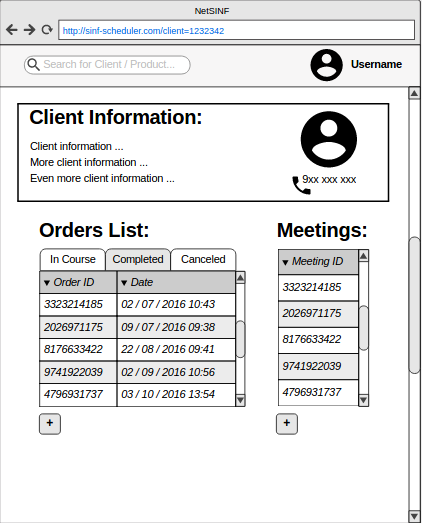
\includegraphics[width=9cm, height = 10.5cm]{SINF_clientpage.png}
  \caption{Core View da página de cliente.}
  \label{uml}
\end{figure}

\begin{table}[H]
\centering
\caption{Core View Client Page especificação.}
\label{my-label}
\begin{tabular}{@{}cl@{}}
\toprule
ID CORE VIEW                                                   & CLI\_PAGE                                                                                                                                                                                                                                                                                                                           \\ \midrule
INWARD PATHS                                                   & \begin{tabular}[c]{@{}l@{}}-Homepage;\\ -Meeting Page;\\ -Order Page.\end{tabular}                                                                                                                                                                                                                                            \\ \midrule
OUTWARD PATHS                                                  & \begin{tabular}[c]{@{}l@{}}-Allows the user to see detailed client information;\\ -Displays complete history of pending, completed\\ and canceled orders;\\ -Allows starting a new order with the client;\\ - Display history of meetings with client;\\ -Allows scheduling a new meeting with the client.\end{tabular} \\ \midrule
\begin{tabular}[c]{@{}c@{}}ELEMENTS OF\\ THE CORE\end{tabular} & \begin{tabular}[c]{@{}l@{}}Client Information Summary, Order Information\\ Table, Context Tabs and New Order Button\end{tabular}                                                                                                                                                                                        \\ \bottomrule
\end{tabular}
\end{table}

\subsection{Homepage: Overview of schedule}

\begin{figure}[H]
  \centering
    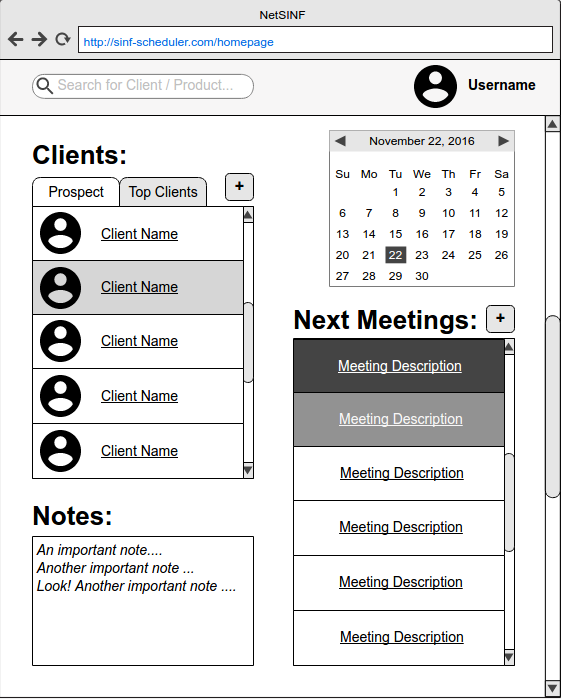
\includegraphics[width=9cm, height = 10.5cm]{SINF_homepage.png}
  \caption{Core View da página inicial.}
  \label{uml}
\end{figure}

\begin{table}[H]
\centering
\caption{Core View Homepage especificação.}
\label{my-label}
\begin{tabular}{@{}cl@{}}
\hline
ID CORE VIEW                                                   & HOM\_PAGE                                                                                                                                                                                                                                                             \\ \midrule
INWARD PATHS                                                   & \begin{tabular}[c]{@{}l@{}}-Sign in;\\ -Home button\end{tabular}                                                                                                                                                                                                         \\ \midrule
OUTWARD PATHS                                                  & \begin{tabular}[c]{@{}l@{}}-Allow user to quickly verify future meetings\\ and take relevant notes if necessary;\\ -Enables scheduling of new meetings with\\ existing clients;\\ -Allows user to add new clients and easily \\ access their information.\end{tabular} \\  \midrule 
\begin{tabular}[c]{@{}c@{}}ELEMENTS OF\\ THE CORE\end{tabular} & \begin{tabular}[c]{@{}l@{}}Clients Grid, Meetings list, Meetings calendar,\\ Note text area\end{tabular}                                                                                                                                                               \\ \bottomrule
\end{tabular}
\end{table}

\subsection{Meeting Page: Overview of meeting}

\begin{figure}[H]
  \centering
    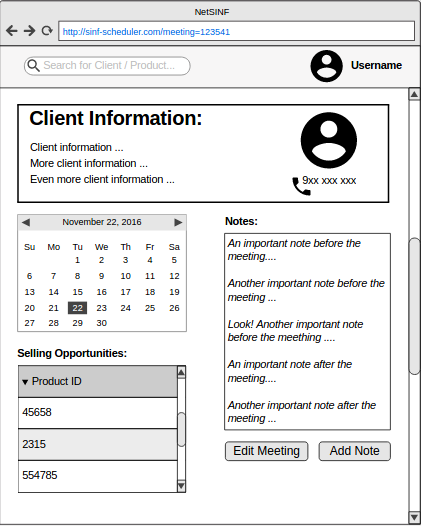
\includegraphics[width=9cm, height = 10.5cm]{SINF_meetingpage.png}
  \caption{Core View da página das reuniões agendadas.}
  \label{uml}
\end{figure}

\begin{table}[H]
\centering
\caption{Core View Meeting Page especificação.}
\label{my-label}
\begin{tabular}{@{}cl@{}}
\toprule
ID CORE VIEW                                                   & VIE\_PAGE                                                                                                                                                                                                                               \\ \midrule
INWARD PATHS                                                   & \begin{tabular}[c]{@{}l@{}}-Homepage;\\ -Client Page.\end{tabular}                                                                                                                                                                      \\ \midrule
OUTWARD PATHS                                                  & \begin{tabular}[c]{@{}l@{}}-Allows the user to see detailed client information;\\ -Allows the user to take relevant notes after the meeting;\\ -Shows the detailed list of selling opportunities proposed\\ to the client.\end{tabular} \\ \midrule
\begin{tabular}[c]{@{}c@{}}ELEMENTS OF\\ THE CORE\end{tabular} & \begin{tabular}[c]{@{}l@{}}Client Information Summary, Meeting Calendar, Notes \\ Text Area and Selling Opportunities List\end{tabular}                                                                                                 \\ \bottomrule
\end{tabular}
\end{table}

\subsection{New Client Page: Create page for new potencial client}

\begin{figure}[H]
  \centering
    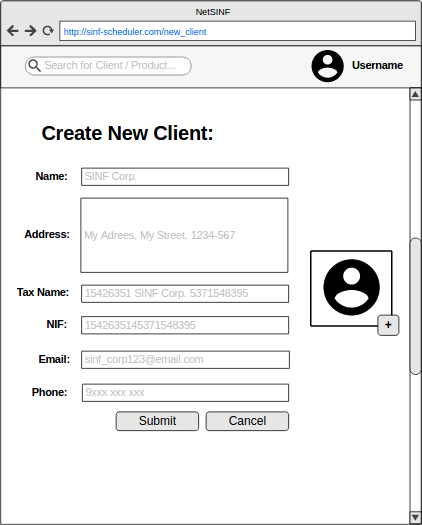
\includegraphics[width=9cm, height = 10.5cm]{SINF_newclient.png}
  \caption{Core View da página para adicionar um cliente.}
  \label{uml}
\end{figure}

\begin{table}[H]
\centering
\caption{Core View New Client especificação.}
\label{my-label}
\begin{tabular}{@{}cl@{}}
\toprule
ID CORE VIEW                                                   & NEW\_CLI                             \\ \midrule
INWARD PATHS                                                   & -Homepage.                           \\  \midrule
OUTWARD PATHS                                                  & -Allows the creation of new clients. \\  \midrule
\begin{tabular}[c]{@{}c@{}}ELEMENTS OF\\ THE CORE\end{tabular} & New Client Form                      \\ \bottomrule
\end{tabular}
\end{table}

\subsection{New Meeting Page: Schedule meeting with client}

\begin{figure}[H]
  \centering
    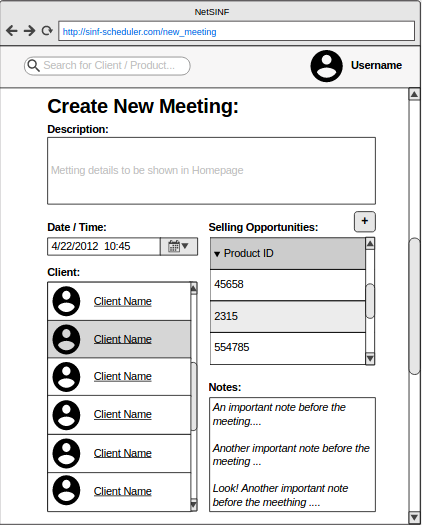
\includegraphics[width=9cm, height = 10.5cm]{SINF_newmeeting.png}
  \caption{Core View da página para adicionar uma reunião.}
  \label{uml}
\end{figure}

\begin{table}[H]
\centering
\caption{Core View New Meeting Page especificação.}
\label{my-label}
\begin{tabular}{@{}cl@{}}
\toprule
ID CORE VIEW                                                   & NEW\_MEE                                                                                                                                                                                                                                                                                          \\ \midrule
INWARD PATHS                                                   & \begin{tabular}[c]{@{}l@{}}-Homepage;\\ -Client Page.\end{tabular}                                                                                                                                                                                                                                \\ \midrule
OUTWARD PATHS                                                  & \begin{tabular}[c]{@{}l@{}}-Enables the scheduling of new meetings with clients;\\ -Verifies if different meetings do not overlap each other;\\ -Enables to select the products to sell and access their \\ respective pages;\\ -Enables to take important notes before the meeting.\end{tabular} \\ \midrule
\begin{tabular}[c]{@{}c@{}}ELEMENTS OF\\ THE CORE\end{tabular} & \begin{tabular}[c]{@{}l@{}}Description Text Area, Meeting Data Picker, Client List\\ and Selling Opportunities List\end{tabular}                                                                                                                                                                  \\ \bottomrule
\end{tabular}
\end{table}

\subsection{New Order Page: Sell products to client}

\begin{figure}[H]
  \centering
    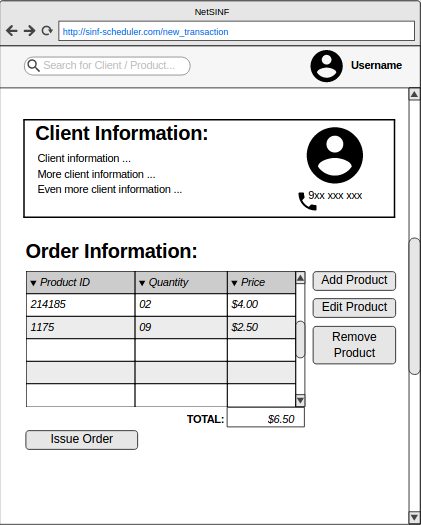
\includegraphics[width=9cm, height = 10.5cm]{SINF_neworder.png}
  \caption{Core View da página para adicionar um pedido de um cliente.}
  \label{uml}
\end{figure}

\begin{table}[H]
\centering
\caption{Core View New Order Page especificação.}
\label{my-label}
\begin{tabular}{@{}cl@{}}
\toprule
ID CORE VIEW                                                   & NEW\_TRA                                                                                                                                       \\ \midrule
INWARD PATHS                                                   & \begin{tabular}[c]{@{}l@{}}-Client Page;\\ -Meeting Page.\end{tabular}                                                                         \\ \midrule
OUTWARD PATHS                                                  & \begin{tabular}[c]{@{}l@{}}-Allows user to see specific information about the client;\\ -Enables the creation of complete orders.\end{tabular} \\ \midrule
\begin{tabular}[c]{@{}c@{}}ELEMENTS OF\\ THE CORE\end{tabular} & \begin{tabular}[c]{@{}l@{}}Client Information Summary, New Order Table and Action\\ Buttons\end{tabular}                                       \\ \bottomrule
\end{tabular}
\end{table}

\subsection{Order Status Page: Overview of order status}

\begin{figure}[H]
  \centering
    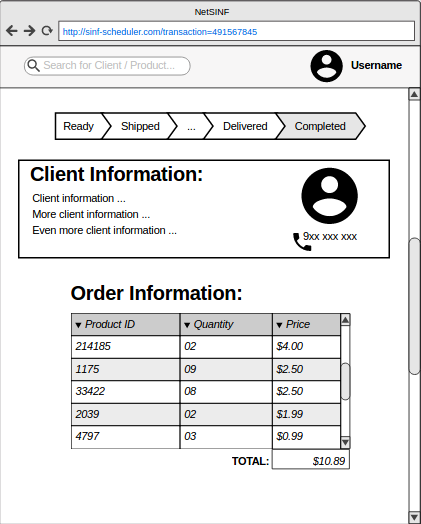
\includegraphics[width=9cm, height = 10.5cm]{SINF_orderpage.png}
  \caption{Core View da página onde se visualiza um pedido de um cliente.}
  \label{uml}
\end{figure}

\begin{table}[H]
\centering
\caption{Core View Order Status Page especificação.}
\label{my-label}
\begin{tabular}{@{}cl@{}}
\toprule
ID CORE VIEW                                                   & TRA\_PAGE                                                                                                                                                                         \\ \midrule
INWARD PATHS                                                   & -Client Page.                                                                                                                                                                     \\ \midrule
OUTWARD PATHS                                                  & \begin{tabular}[c]{@{}l@{}}-Allows user to see the order status;\\ -Enables user to access client information;\\ -Enables user to see detailed information of order.\end{tabular} \\ \midrule
\begin{tabular}[c]{@{}c@{}}ELEMENTS OF\\ THE CORE\end{tabular} & \begin{tabular}[c]{@{}l@{}}Status Bar, Client Information Summary and Order\\ Information Table\end{tabular}                                                                      \\ \bottomrule
\end{tabular}
\end{table}

\subsection{Product Page: Overview of product}

\begin{figure}[H]
  \centering
    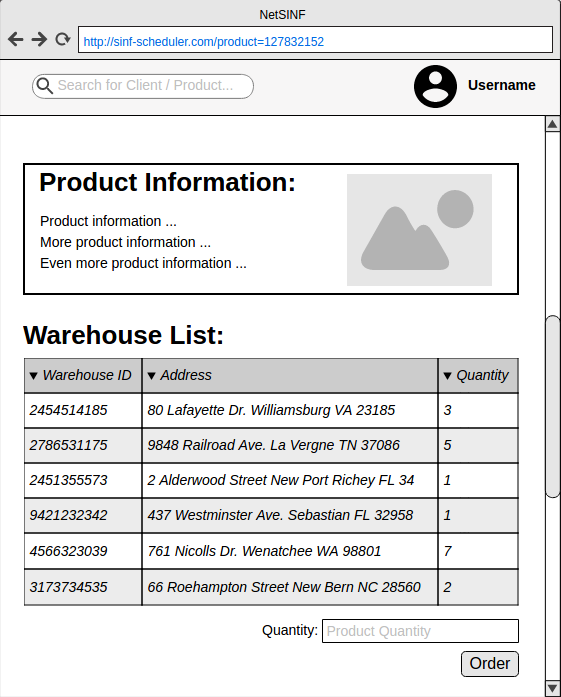
\includegraphics[width=9cm, height = 10.5cm]{SINF_productpage.png}
  \caption{Core View da página de um produto e a sua disponibilidade em cada armazém.}
  \label{uml}
\end{figure}

\begin{table}[H]
\centering
\caption{Core View Product Page especificação.}
\label{my-label}
\begin{tabular}{@{}cl@{}}
\toprule
ID CORE VIEW                                                   & PRO\_PAGE                                                                                                                                                                                                                                                                   \\ \midrule
INWARD PATHS                                                   & \begin{tabular}[c]{@{}l@{}}-Order Page;\\ -Meeting Page.\end{tabular}                                                                                                                                                                                                 \\ \midrule
OUTWARD PATHS                                                  & \begin{tabular}[c]{@{}l@{}}-Enables the user to see detailed information about a product;\\ -Enables the user to check availability of a product in several\\ warehouses and respective stock;\\ -Enables user to request a defined quantity of product units.\end{tabular} \\ \midrule
\begin{tabular}[c]{@{}c@{}}ELEMENTS OF\\ THE CORE\end{tabular} & Product Information Summary and Warehouse Table                                                                                                                                                                                                                             \\ \bottomrule
\end{tabular}
\end{table}

\section{Interoperabilidade}

\subsection{Clientes}

\begin{table}[H]
\centering
\caption{Tabela do método get\_client.}
\label{my-label}
\begin{tabular}{|c|l|}
\hline 
\textbf{Webservice ID}                     & \multicolumn{1}{c|}{get\_client}                                                                                                                                                                                        \\ \hline
\multicolumn{1}{|l|}{\textbf{Description}} & Retorna a informação de um cliente específico.                                                                                                                                                                                    \\ \hline
\textbf{Core Views}                        & CLI\_PAGE                                                                                                                                                                                                                          \\ \hline
\textbf{Path}                              & \url{http://<domain>/api/client=<clientID>}                                                                                                                                                          \\ \hline
\textbf{Verb}                              & \multicolumn{1}{c|}{GET}                                                                                                                                                                                                \\ \hline
\textbf{Input}                             & \multicolumn{1}{c|}{clientID}                                                                                                                                                                                           \\ \hline
\textbf{Output}                            & \begin{tabular}[c]{@{}l@{}}\{\\      "id": "EFACSA",\\      "nome": "EFACEC",\\      "nome\_fiscal": "EFACEC SA",\\ \\      "morada": "Porto",\\      "telefone": 969509655,\\      "contribuinte": 989922455\\ \}\end{tabular} \\ \hline
\end{tabular}
\end{table}

\begin{table}[H]
\centering
\caption{Tabela do método get\_all\_clients.}
\label{my-label}
\begin{tabular}{|c|l|}
\hline 
\textbf{Webservice ID}                     & \multicolumn{1}{c|}{get\_all\_clients}                                                                                                                                                                                        \\ \hline
\multicolumn{1}{|l|}{\textbf{Description}} & Retorna todos os clientes.                                                                                                                                                                                    \\ \hline
\textbf{Core Views}                        & HOM\_PAGE                                                                                                                                                                                                                          \\ \hline
\textbf{Path}                              & \url{http://<domain>/api/user=<userID>}                                                                                                                                                          \\ \hline
\textbf{Verb}                              & \multicolumn{1}{c|}{GET}                                                                                                                                                                                                \\ \hline
\textbf{Input}                             & \multicolumn{1}{c|}{userID}                                                                                                                                                                                           \\ \hline
\textbf{Output}                            & \begin{tabular}[c]{@{}l@{}}\{  "Clientes": [ \\ \{ "id": "EFACSA",\\     "nome": "EFACEC",\\     "nome\_fiscal": "EFACEC SA",\\ \\      "morada": "Porto",\\      "telefone": 969509655,\\      "contribuinte": 989922455\\ \}, \\ \{ \\ "id":  "LIMA", \\ "nome":  "Empreendimentos do Lima", \\ "nome\_fiscal": "Empreendimentos do Lima, Lda", \\ "morada": "Bairro PSP", \\ "telefone": , \\ "contribuinte": 202075133 \\ \}  \\ ]\}
\end{tabular} \\ \hline
\end{tabular}
\end{table}


\begin{table}[H]
\centering
\caption{Tabela do método add\_client.}
\label{my-label}
\begin{tabular}{|c|l|}
\hline 
\textbf{Webservice ID}                     & \multicolumn{1}{c|}{add\_client}                                                                                                                                                                                        \\ \hline
\multicolumn{1}{|l|}{\textbf{Description}} & Adiciona um cliente.                                                                                                                                                                                    \\ \hline
\textbf{Core Views}                        & NEW\_CLI                                                                                                                                                                                                                         \\ \hline
\textbf{Path}                              & \url{http://<domain>/api}                                                                                                                                                          \\ \hline
\textbf{Verb}                              & \multicolumn{1}{c|}{POST}                                                                                                                                                                                                \\ \hline
\textbf{Input}                             & \multicolumn{1}{c|}{nome, nome\_fiscal, email, morada, telefone, contribuinte}                                                                                                                                                                                           \\ \hline
\textbf{Output}                            & \begin{tabular}[c]{@{}l@{}}\{\\  "resultado": "OK" \\ \}\end{tabular} \\ \hline
\end{tabular}
\end{table}

\subsection{Reuniões}

\begin{table}[H]
\centering
\caption{Tabela do método get\_meetings.}
\label{my-label}
\begin{tabular}{|c|l|}
\hline 
\textbf{Webservice ID}                     & \multicolumn{1}{c|}{get\_meetings}                                                                                                                                                                                        \\ \hline
\multicolumn{1}{|l|}{\textbf{Description}} & Retorna as reuniões.                                                                                                                                                                                    \\ \hline
\textbf{Core Views}                        & HOM\_PAGE
\\ \hline
\textbf{Path}                              & \url{http://<domain>/api/user=<userID>}                                                                                                                                                          \\ \hline
\textbf{Verb}                              & \multicolumn{1}{c|}{GET}                                                                                                                                                                                                \\ \hline
\textbf{Input}                             & \multicolumn{1}{c|}{userID}                                                                                                                                                                                           \\ \hline
\textbf{Output}                            & \begin{tabular}[c]{@{}l@{}}\{ "Reunioes": [ \\ \{\\  "descricao": "Discussão dos novos produtos da empresa.", \\ 
"data": 29/10/2016, \\ "tempo": 16h00, \\ \begin{tabular}[c]{@{}l@{}}"notas": "Não esquecer de mencionar a promoção em vigor \\ para a compra de 100 unidades." \\ \}, \end{tabular}  
\\
 \begin{tabular}[c]{@{}l@{}} \{ \\  "descricao": "Discussão de uma parceria com a equipa de marketing.", \\ 
"data": 30/10/2016, \\ "tempo": 10h00, \\ "notas": "Nome do representante é João Figueiredo." \\ \} ] \end{tabular}  \end{tabular} \\ \hline
\end{tabular}
\end{table}

\begin{table}[H]
\centering
\caption{Tabela do método add\_meeting.}
\label{my-label}
\begin{tabular}{|c|l|}
\hline 
\textbf{Webservice ID}                     & \multicolumn{1}{c|}{add\_meeting}                                                                                                                                                                                        \\ \hline
\multicolumn{1}{|l|}{\textbf{Description}} & Adiciona uma reunião.                                                                                                                                                                                    \\ \hline
\textbf{Core Views}                        & NEW\_MEE
\\ \hline
\textbf{Path}                              & \url{http://<domain>/api}                                                                                                                                                          \\ \hline
\textbf{Verb}                              & \multicolumn{1}{c|}{POST}                                                                                                                                                                                                \\ \hline
\textbf{Input}                             & \multicolumn{1}{c|}{descricao, data, tempo, notas}                                                                                                                                                                                           \\ \hline
\textbf{Output}                            & \begin{tabular}[c]{@{}l@{}}\{\\  "resultado": "OK" \\ \}\end{tabular} \\ \hline
\end{tabular}
\end{table}

\begin{table}[H]
\centering
\caption{Tabela do método edit\_meeting.}
\label{my-label}
\begin{tabular}{|c|l|}
\hline 
\textbf{Webservice ID}                     & \multicolumn{1}{c|}{edit\_meeting}                                                                                                                                                                                        \\ \hline
\multicolumn{1}{|l|}{\textbf{Description}} & Edita uma reunião.                                                                                                                                                                                    \\ \hline
\textbf{Core Views}                        & 
\\ \hline
\textbf{Path}                              & \url{http://<domain>/api/meeting}                                                                                                                                                          \\ \hline
\textbf{Verb}                              & \multicolumn{1}{c|}{PUT}                                                                                                                                                                                                \\ \hline
\textbf{Input}                             & \multicolumn{1}{c|}{descricao, data, tempo, notas}                                                                                                                                                                                           \\ \hline
\textbf{Output}                            & \begin{tabular}[c]{@{}l@{}}\{\\  "resultado": "OK" \\ \}\end{tabular} \\ \hline
\end{tabular}
\end{table}

\begin{table}[H]
\centering
\caption{Tabela do método delete\_meeting.}
\label{my-label}
\begin{tabular}{|c|l|}
\hline 
\textbf{Webservice ID}                     & \multicolumn{1}{c|}{delete\_meeting}                                                                                                                                                                                        \\ \hline
\multicolumn{1}{|l|}{\textbf{Description}} & Apaga uma reunião.                                                                                                                                                                                    \\ \hline
\textbf{Core Views}                        & 
\\ \hline
\textbf{Path}                              & \url{http://<domain>/api/meeting=<meetingID>}                                                                                                                                                          \\ \hline
\textbf{Verb}                              & \multicolumn{1}{c|}{DELETE}                                                                                                                                                                                                \\ \hline
\textbf{Input}                             & \multicolumn{1}{c|}{meetingID}                                                                                                                                                                                           \\ \hline
\textbf{Output}                            & \begin{tabular}[c]{@{}l@{}}\{\\  "resultado": "OK" \\ \}\end{tabular} \\ \hline
\end{tabular}
\end{table}

\subsection{Armazéns}

\begin{table}[H]
\centering
\caption{Tabela do método get\_warehouse.}
\label{my-label}
\begin{tabular}{|c|l|}
\hline
\textbf{Webservice ID}                     & \multicolumn{1}{c|}{get\_warehouse}                                                                                                                                                                                        \\ \hline
\multicolumn{1}{|l|}{\textbf{Description}} & Retorna a informação dos armazens.
 \\ \hline
\textbf{Core Views}                        & \multicolumn{1}{c|}{PRO\_PAGE}                                                                                                                                                                                                                        \\ \hline
\textbf{Path}                              & \url{http://<domain>/api/warehouse=<warehouseID>}                                                                                                                                                          \\ \hline
\textbf{Verb}                              & \multicolumn{1}{c|}{GET}                                                                                                                                                                                                \\ \hline
\textbf{Input}                             & \multicolumn{1}{c|}{warehouseID}                                                                                                                                                                                           \\ \hline
\textbf{Output}                            & \begin{tabular}[c]{@{}l@{}}\{\\      "name": "ARMAZ",\\     "morada": "warehouse location",\\    "contacto": "warehouse contact"\\ \}\end{tabular} \\ \hline
\end{tabular}
\end{table}

\subsection{Transações}

\begin{table}[H]
	\centering
	\caption{Tabela do método get\_transaction.}
	\label{my-label}
	\begin{tabular}{|c|l|}
		\hline
		\textbf{Webservice ID}                     & \multicolumn{1}{c|}{get\_transaction}                                                                                                                                                                                        \\ \hline
		\multicolumn{1}{|l|}{\textbf{Description}} & Retorna a transação.
 \\ \hline
		\textbf{Core Views}                        & \multicolumn{1}{c|}{TRA\_PAGE}                                                                                                                                                                                                                        \\ \hline
		\textbf{Path}                              & \url{http://<domain>/api/transaction=<transactionID>}                                                                                                                                                          \\ \hline
		\textbf{Verb}                              & \multicolumn{1}{c|}{GET}                                                                                                                                                                                                \\ \hline
		\textbf{Input}                             & \multicolumn{1}{c|}{transactionID}                                                                                                                                                                                           \\ \hline
		\textbf{Output}                            & \begin{tabular}[c]{@{}l@{}}\{\\      "clienteID": "EFACSA",\\     "repvendaID": "VENDEDOR",\\    "produtos": [\{ "produtoID": 243,\\ "preco": 22.3,\\ "iva": 21,\\ "desconto": 0\},\\ ...],\\ "data": "2016-10-09 15:12:23" \}\end{tabular} \\ \hline
	\end{tabular}
\end{table}


\begin{table}[H]
	\centering
	\caption{Tabela do método post\_transaction.}
	\label{my-label}
	\begin{tabular}{|c|l|}
		\hline
		\textbf{Webservice ID}                     & \multicolumn{1}{c|}{post\_transaction}                                                                                                                                                                                        \\ \hline
		\multicolumn{1}{|l|}{\textbf{Description}} & Adiciona uma transação.                                                                                                                                                                                    \\ \hline
		\textbf{Core Views}                        & \multicolumn{1}{c|}{NEW\_TRA}                                                                                                                                                                                                                        \\ \hline
		\textbf{Path}                              & \url{http://<domain>/api/transaction}                                                                                                                                                          \\ \hline
		\textbf{Verb}                              & \multicolumn{1}{c|}{POST}                                                                                                                                                                                                \\ \hline
		\textbf{Input}                             & \multicolumn{1}{c|}{clienteID, repvendaID, listaProdutos}                                                                                                                                                                                           \\ \hline
		\textbf{Output}                            & \begin{tabular}[c]{@{}l@{}}\{\\  "resultado": "OK" \\ \}\end{tabular} \\ \hline
	\end{tabular}
\end{table}

\subsection{Artigos}

\begin{table}[H]
	\centering
	\caption{Tabela do método get\_article.}
	\label{my-label}
	\begin{tabular}{|c|l|}
		\hline
		\textbf{Webservice ID}                     & \multicolumn{1}{c|}{get\_article}                                                                                                                                                                                        \\ \hline
		\multicolumn{1}{|l|}{\textbf{Description}} & Retorna um artigo.                                                                                                                                                                                    \\ \hline
		\textbf{Core Views}                        & \multicolumn{1}{c|}{PRO\_PAGE}                                                                                                                                                                                                                        \\ \hline
		\textbf{Path}                              & \url{http://<domain>/api/article=<articleID>}                                                                                                                                                          \\ \hline
		\textbf{Verb}                              & \multicolumn{1}{c|}{GET}                                                                                                                                                                                                \\ \hline
		\textbf{Input}                             & \multicolumn{1}{c|}{articleID}                                                                                                                                                                                           \\ \hline
		\textbf{Output}                            & \begin{tabular}[c]{@{}l@{}}\{\\  "nome": "nome artigo",\\ "descricao": "descricao artigo",\\ "preco\_atual": 12.5,\\ "iva\_atual": 13 \\ \}\end{tabular} \\ \hline
	\end{tabular}
\end{table}

\subsection{Administrador}

\begin{table}[H]
	\centering
	\caption{Tabela do método get\_product\_stats.}
	\label{my-label}
	\begin{tabular}{|c|l|}
		\hline
		\textbf{Webservice ID}                     & \multicolumn{1}{c|}{get\_product\_stats}                                                                                                                                                                                        \\ \hline
		\multicolumn{1}{|l|}{\textbf{Description}} & Retorna as estatísticas de um produto num certo intervalo de tempo.                                                                                                                                                                                    \\ \hline
		\textbf{Core Views}                        & \multicolumn{1}{c|}{}                                                                                                                                                                                                                        \\ \hline
		\textbf{Path}                              & \url{http://<domain>/api/article=<articleID>&time=<timePeriod>}                                                                                                                                                          \\ \hline
		\textbf{Verb}                              & \multicolumn{1}{c|}{GET}                                                                                                                                                                                                \\ \hline
		\textbf{Input}                             & \multicolumn{1}{c|}{articleID, time\_period}                                                                                                                                                                                           \\ \hline
		\textbf{Output}                            & \begin{tabular}[c]{@{}l@{}}\{\\  "nome": "nome artigo",\\ "vendas": 10000 \\ \}\end{tabular} \\ \hline
	\end{tabular}
\end{table}

\begin{table}[H]
	\centering
	\caption{Tabela do método get\_all\_product\_stats.}
	\label{my-label}
	\begin{tabular}{|c|l|}
		\hline
		\textbf{Webservice ID}                     & \multicolumn{1}{c|}{get\_all\_product\_stats}                                                                                                                                                                                        \\ \hline
		\multicolumn{1}{|l|}{\textbf{Description}} & \begin{tabular}[c]{@{}l@{}}  Retorna estatísticas do número de produtos mais vendidos \\ no intervalo de tempo especificado.                                                                                                                                                                                   
	\end{tabular} \\ \hline
		\textbf{Core Views}                        & \multicolumn{1}{c|}{}                                                                                                                                                                                                                        \\ \hline
		\textbf{Path}                              & \url{http://<domain>/api/article=<articleID>&time=<timePeriod>&nr=<nrP>}                                                                                                                                                                                                                                                             
\\  \hline
		\textbf{Verb}                              & \multicolumn{1}{c|}{GET}                                                                                                                                                                                                \\ \hline
		\textbf{Input}                             & \multicolumn{1}{c|}{articleID, time\_period, nrProducts}                                                                                                                                                                                           \\ \hline
		\textbf{Output}                            & \begin{tabular}[c]{@{}l@{}}\{\\  "artigos": [ \\ \{ "nome": "CloroX",\\ "vendas": 10000 \}, \\  \{ "nome": "Flit",\\ "vendas": 5000 \}  ] \\ \}\end{tabular} \\ \hline
	\end{tabular}
\end{table}

\begin{table}[H]
	\centering
	\caption{Tabela do método get\_salesRep\_stats.}
	\label{my-label}
	\begin{tabular}{|c|l|}
		\hline
		\textbf{Webservice ID}                     & \multicolumn{1}{c|}{get\_salesRep\_stats}                                                                                                                                                                                        \\ \hline
		\multicolumn{1}{|l|}{\textbf{Description}} & \begin{tabular}[c]{@{}l@{}}  Retorna estatísticas de vendas de um vendedore específico.               
	\end{tabular} \\ \hline
		\textbf{Core Views}                        & \multicolumn{1}{c|}{}                                                                                                                                                                                                                        \\ \hline
		\textbf{Path}                              & \url{http://<domain>/api/salesRep=<salesRepID>&time=<timePeriod>}                                                                                                                                                                                                                                                             
\\  \hline
		\textbf{Verb}                              & \multicolumn{1}{c|}{GET}                                                                                                                                                                                                \\ \hline
		\textbf{Input}                             & \multicolumn{1}{c|}{salesRepID, time\_period}                                                                                                                                                                                           \\ \hline
		\textbf{Output}                            & \begin{tabular}[c]{@{}l@{}} \{ "nome": "João Claro",\\ "vendas": 10000 \}\end{tabular}  \\ \hline
	\end{tabular}
\end{table}

\begin{table}[H]
	\centering
	\caption{Tabela do método get\_all\_salesRep\_stats.}
	\label{my-label}
	\begin{tabular}{|c|l|}
		\hline
		\textbf{Webservice ID}                     & \multicolumn{1}{c|}{get\_all\_salesRep\_stats}                                                                                                                                                                                        \\ \hline
		\multicolumn{1}{|l|}{\textbf{Description}} & \begin{tabular}[c]{@{}l@{}}  Retorna estatísticas de vendas do número de vendedores especificado.               
	\end{tabular} \\ \hline
		\textbf{Core Views}                        & \multicolumn{1}{c|}{}                                                                                                                                                                                                                        \\ \hline
		\textbf{Path}                              & \url{http://<domain>/api/salesRep=<salesRepID>&time=<timePeriod>&nr=<nrS>}                                                                                                                                                                                                                                                             
\\  \hline
		\textbf{Verb}                              & \multicolumn{1}{c|}{GET}                                                                                                                                                                                                \\ \hline
		\textbf{Input}                             & \multicolumn{1}{c|}{salesRepID, time\_period, nrSalesRep}                                                                                                                                                                                           \\ \hline
		\textbf{Output}                            & \begin{tabular}[c]{@{}l@{}}\{\\  "vendedores": [ \\ \{ "nome": "João Claro",\\ "vendas": 10000 \}, \\  \{ "nome": "Joana Cabral",\\ "vendas": 3000 \}  ] \\ \}\end{tabular}  \\ \hline
	\end{tabular}
\end{table}



\section{Conclusão}
\justify\normalsize
Finda esta fase, consideram-se atingidos os objetivos definidos para esta primeira fase: foi feita a descrição do projeto – uma aplicação web que oferecerá funcionalidades de uma solução SFA. Enumeraram-se as funcionalidades a implementar e identificaram-se os pontos de ligação com o ERP Primavera.

\bibliography{title_page_1}
\bibliographystyle{plain}

\end{titlepage}
\end{document}